\documentclass{article}

\title{Intersection of lines}

\usepackage{tikz}
\usepackage{amsmath}
\usepackage{amsthm}

\newtheorem{theorem}{Theorem}

\begin{document}
\maketitle

\begin{abstract}
This document outlines a method for determining whether the intersection of two lines falls within a circle.
\end{abstract}

\section{Setup}
Consider two lines each defined by two points on a circle, $P_1$ and $P_2$
and $Q_1$ and $Q_2$.

\vspace{1pc}

\begin{figure}[h]
\centering
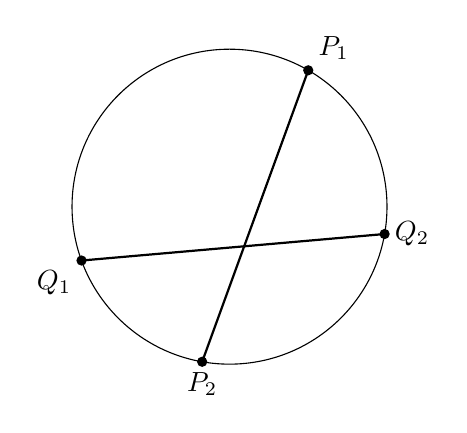
\begin{tikzpicture}[scale=2,>=latex]
    % \draw [<->,gray] (1.2,0) -- (0,0) -- (0,1.2);
    \draw (0,0) circle [radius=1];
    \draw [fill,thick] (60:1) circle [radius=.025]
                        node [above right] {$P_1$}
                  -- (-100:1) circle [radius=.025]
                              node [below] {$P_2$};
    
    \draw [fill,thick] (-10:1) circle [radius=.025]
                        node [right] {$Q_2$}
                  -- (-160:1) circle [radius=.025]
                              node [below left] {$Q_1$};
\end{tikzpicture}
\caption{Two lines}
\end{figure}

These lines can obviously intersect or not. This intersection can be checked 
without reference to the lines, but by simply looking at the angles of the points.

If $P_1$ and $P_2$ are ``next to'' each other, that is, there i no point between them, then they do not intersect any point.
On the other hand, if there is a point between them, but not that points counterpart, then that point's line will intersect it.

\pagebreak

\begin{figure}[h]
\centering
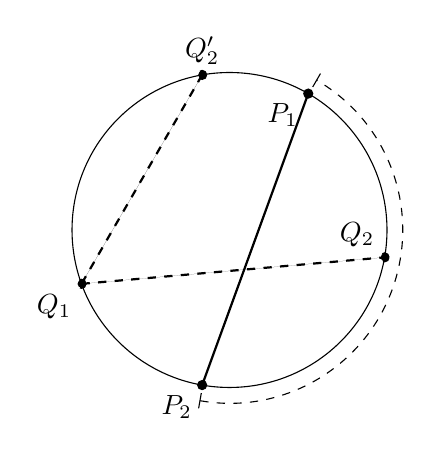
\begin{tikzpicture}[scale=2,>=latex]
    % \draw [<->,gray] (1.2,0) -- (0,0) -- (0,1.2);
    \draw (0,0) circle [radius=1];
    \draw [fill,thick] (60:1) circle [radius=.025]
                        node [below left] {$P_1$}
                  -- (-100:1) circle [radius=.025]
                              node [below left] {$P_2$};
    
    \draw [fill,thick,dashed] (100:1) circle [radius=.025]
                                      node [above] {$Q_2^{\prime}$}
                          -- (-160:1) circle [radius=.025]
                                      node [below left] {$Q_1$}       
                          -- (-10:1) circle [radius=.025]
                                     node [above left] {$Q_2$};
    \draw[|-|,thin,dashed] (-100:1.1) arc (-100:60:1.1);
\end{tikzpicture}
\caption{Intersecting vs. Non-intersecting lines}

\end{figure}

We can see that the line $\overline{Q_1 Q_2}$ intersects $\overline{P_1 P_2}$,
while $\overline{Q_1 Q_2^{\prime}}$ does not. In cact, any placement of $Q_2$ within the dashed interval
will result in an intersection, while any outside will not. This, in order to check fot intersection, it is sufficient to check the sequence of angles.

\section{Method}
\textbf{TODO}

\vspace{2in}

\renewcommand\qedsymbol{\framebox{\textit{\small libtards destroyed}}}

\begin{theorem}
    ur mom gay lol
\end{theorem}
\begin{proof}
    \begin{enumerate}
        \item \textbf{FACTS\footnote{Shapiro, Benjamin, \textit{SJWs DESTROYED compilation, part \#23}, YouTube, 2013}}
        \item \textbf{LOGIC}
    \end{enumerate}
\end{proof}

\end{document}